\begin{frame}
  \begin{center}
    {\bf Hands-on: Exploiting Weaknesses in RSA}\\
    {\bf -- enter D4-project --}\\
  \end{center}
\end{frame}

\begin{frame}
        \frametitle{Problem statement}
        \begin{itemize}
                \item CSIRTs (or private organisations) build their {\bf own honeypot, honeynet or blackhole monitoring network}
                \item Designing, managing and operating such infrastructure is a tedious and resource intensive task
                \item {\bf Automatic sharing} between monitoring networks from different organisations is missing
                \item Sensors and processing are often seen as blackbox or difficult to audit

        \end{itemize}
\end{frame}

\begin{frame}
 \frametitle{Objective}
 \begin{itemize}
         \item Based on our experience with
           MISP\footnote{\url{https://github.com/MISP/MISP}} where sharing
           played an important role, we transpose the model in D4 project
         \item Keeping the protocol and code base {\bf simple and minimal}
         \item Allowing every organisation to {\bf control and audit their own sensor network}
         \item Extending D4 or {\bf encapsulating legacy monitoring protocols} must be as simple as possible
         \item Ensuring that the sensor server has {\bf no control on the sensor} (unidirectional streaming)
         \item Don't force users to use dedicated sensors and allow {\bf flexibility of sensor support} (software, hardware, virtual)

 \end{itemize}
\end{frame}

\begin{frame}
\frametitle{D4 Overview}
        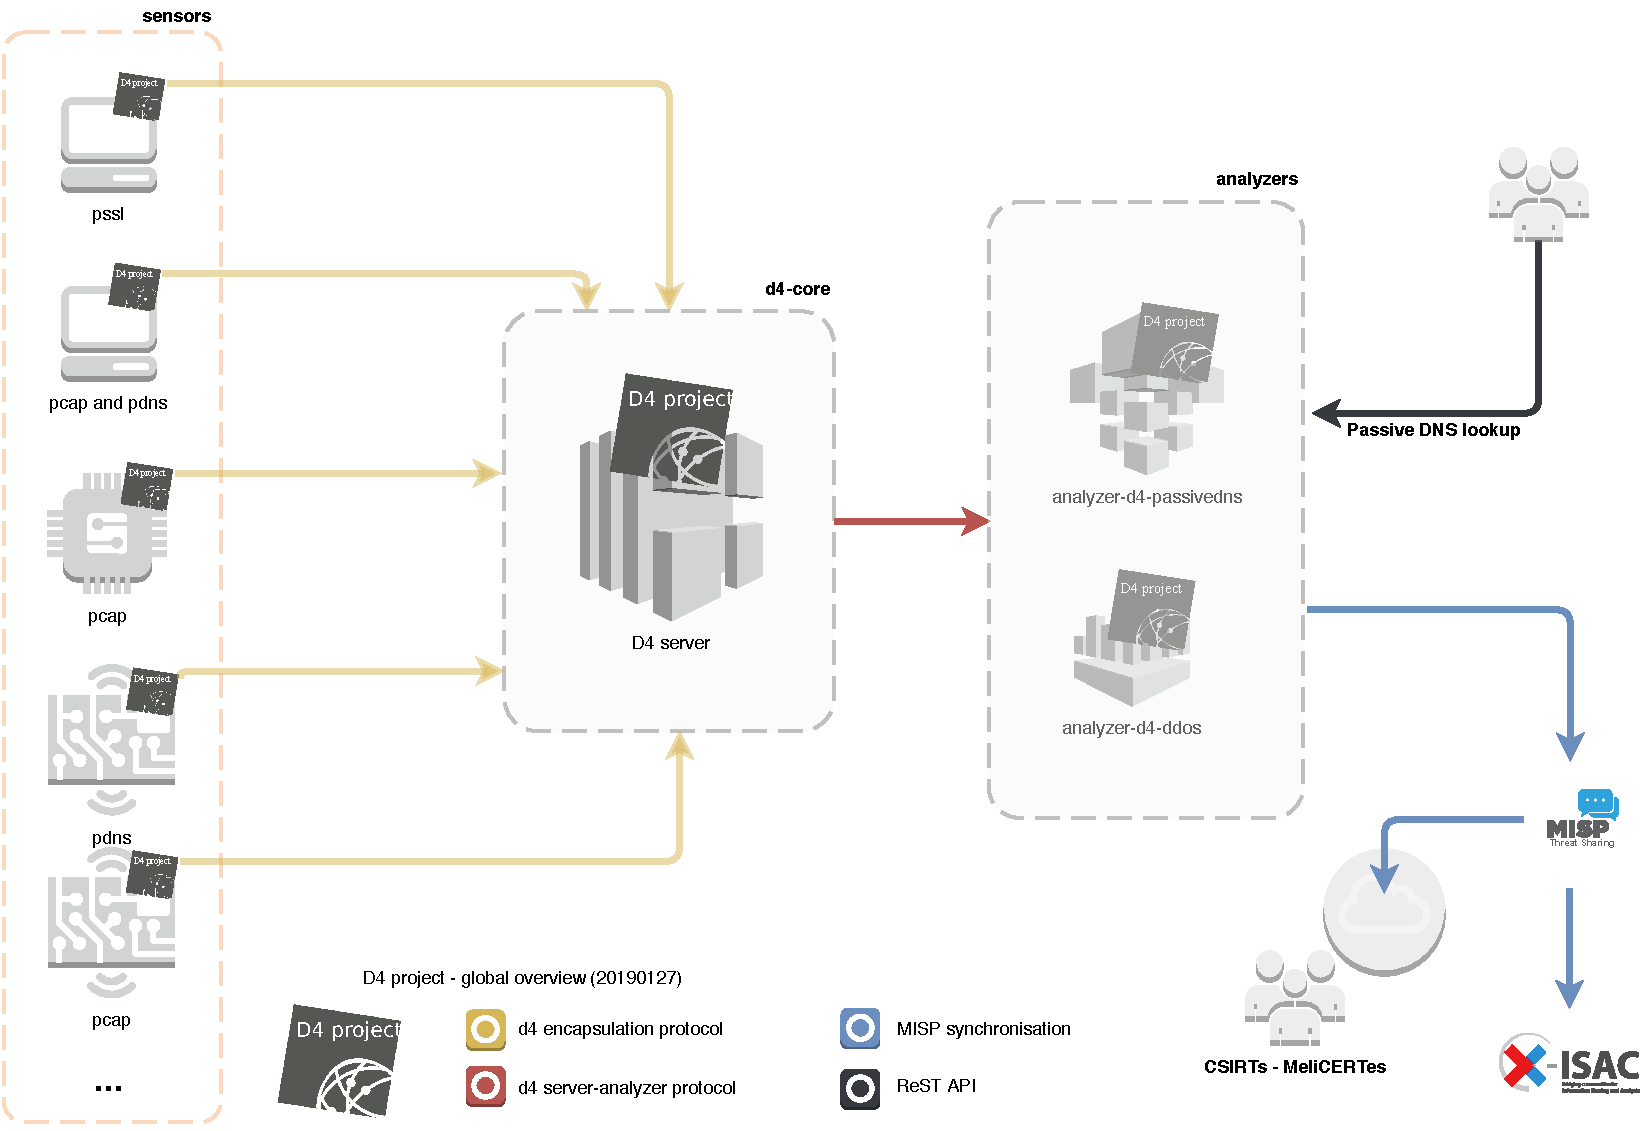
\includegraphics[scale=0.38]{d4-overview.pdf}
\end{frame}


\begin{frame}
\frametitle{D4 Overview - Connecting Sensor Networks}
        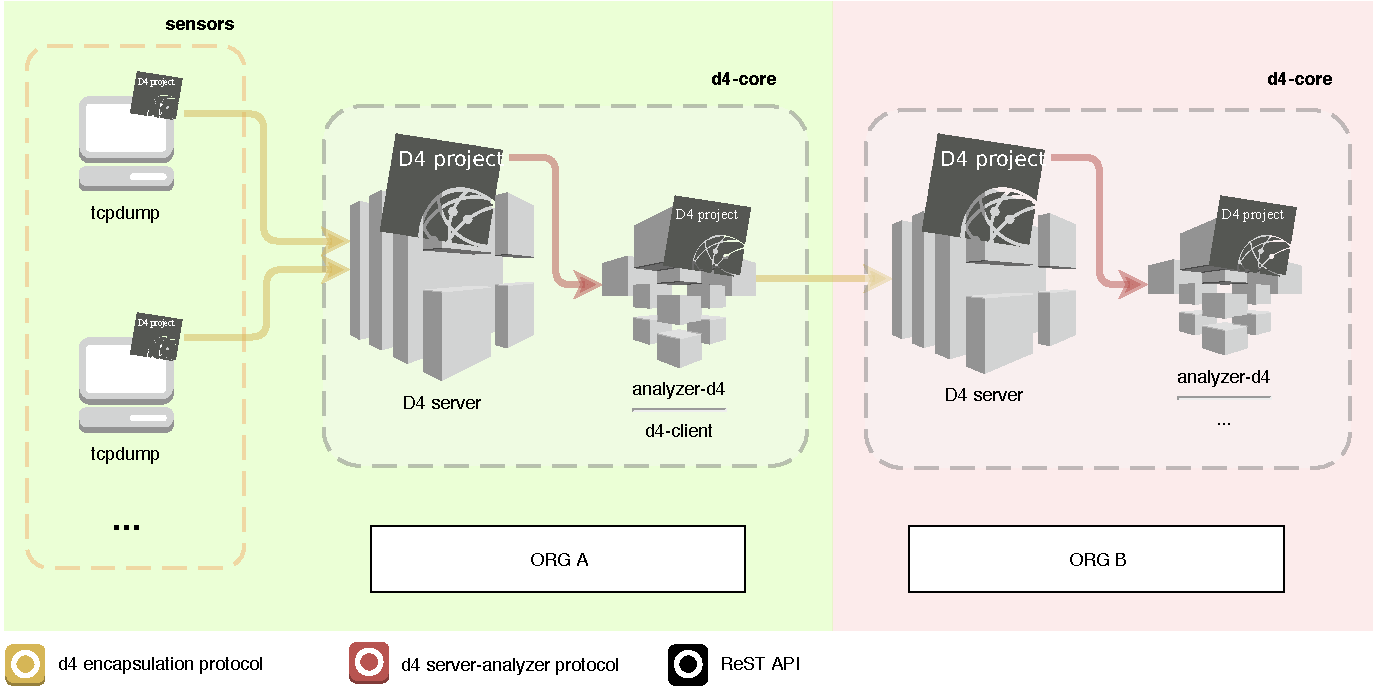
\includegraphics[scale=0.46]{mixing-d4-1.pdf}
\end{frame}
